\chapter{Software Defined Networking}\label{software-defined-networking}

\section{SD Review}\label{sd-review}

\begin{itemize}
\tightlist
\item
  SOFTWARE DEFINED NETWORKING (SDN) is an approach to networking that
  centralizes the control plane into an application called a
  \emph{controller}
\item
  Traditional control planes use a distributed architecture
\item
  A SDN controller centralizes control plane functions like calculating
  routes
\item
  The controller can interact programmatically with the network devices
  using APIs
\item
  The SBI (South Bound Interface) is used for communications between the
  controller and the network device it controls
\item
  The NBI (North Bound Interface) is what allows us to interact with the
  controller with our scripts and applications
\end{itemize}

\section{SDN Architecture}\label{sdn-architecture}

\begin{figure}
\centering
\pandocbounded{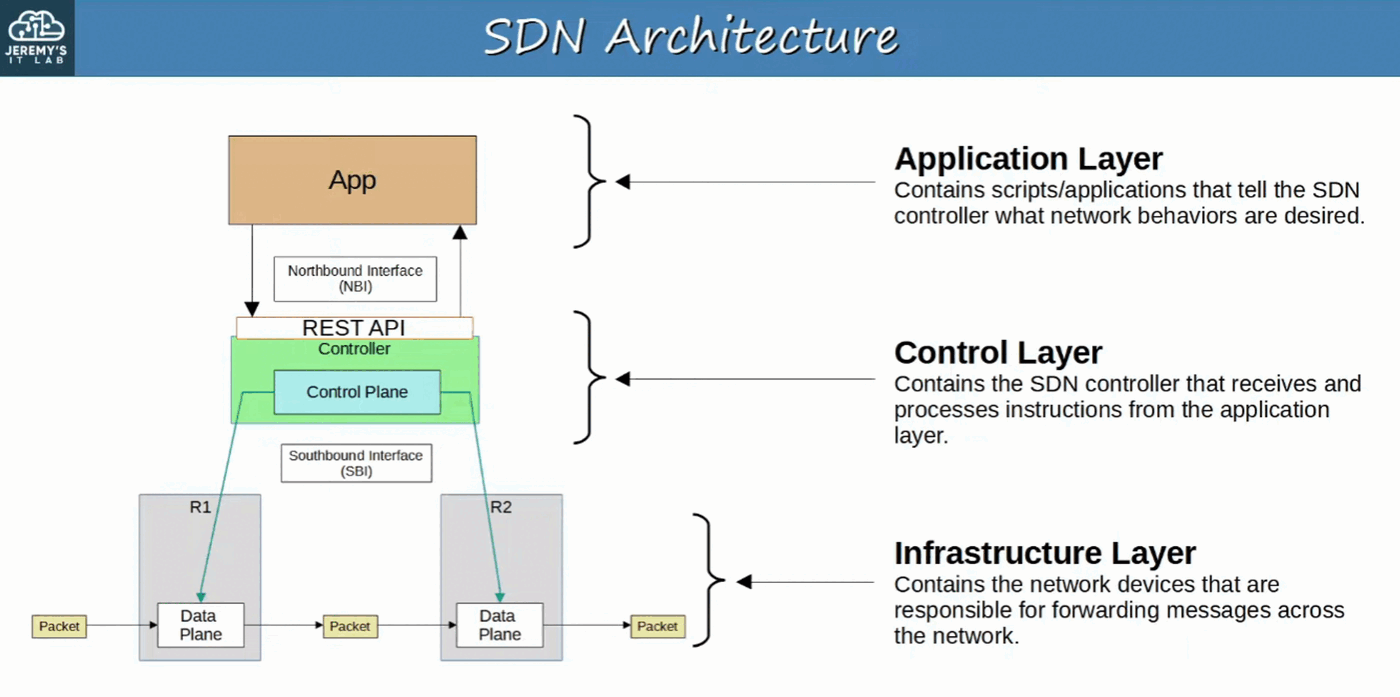
\includegraphics[keepaspectratio,alt={image}]{images/65-software-defined-networking/img-001.png}}
\end{figure}

\section{Cisco SD-Access}\label{cisco-sd-access}

\begin{itemize}
\tightlist
\item
  Cisco SD-ACCESS is Cisco's SDN solution for automating campus LANs

  \begin{itemize}
  \tightlist
  \item
    ACI (Application Centric Infrastructure) is their SDN solution for
    automating data center networks
  \item
    SD-WAN is their SDN solution for automating WANs
  \end{itemize}
\item
  Cisco DNA (Digital Network Architecture) Center is the controller at
  the center of SD-Access
\end{itemize}

\begin{figure}
\centering
\pandocbounded{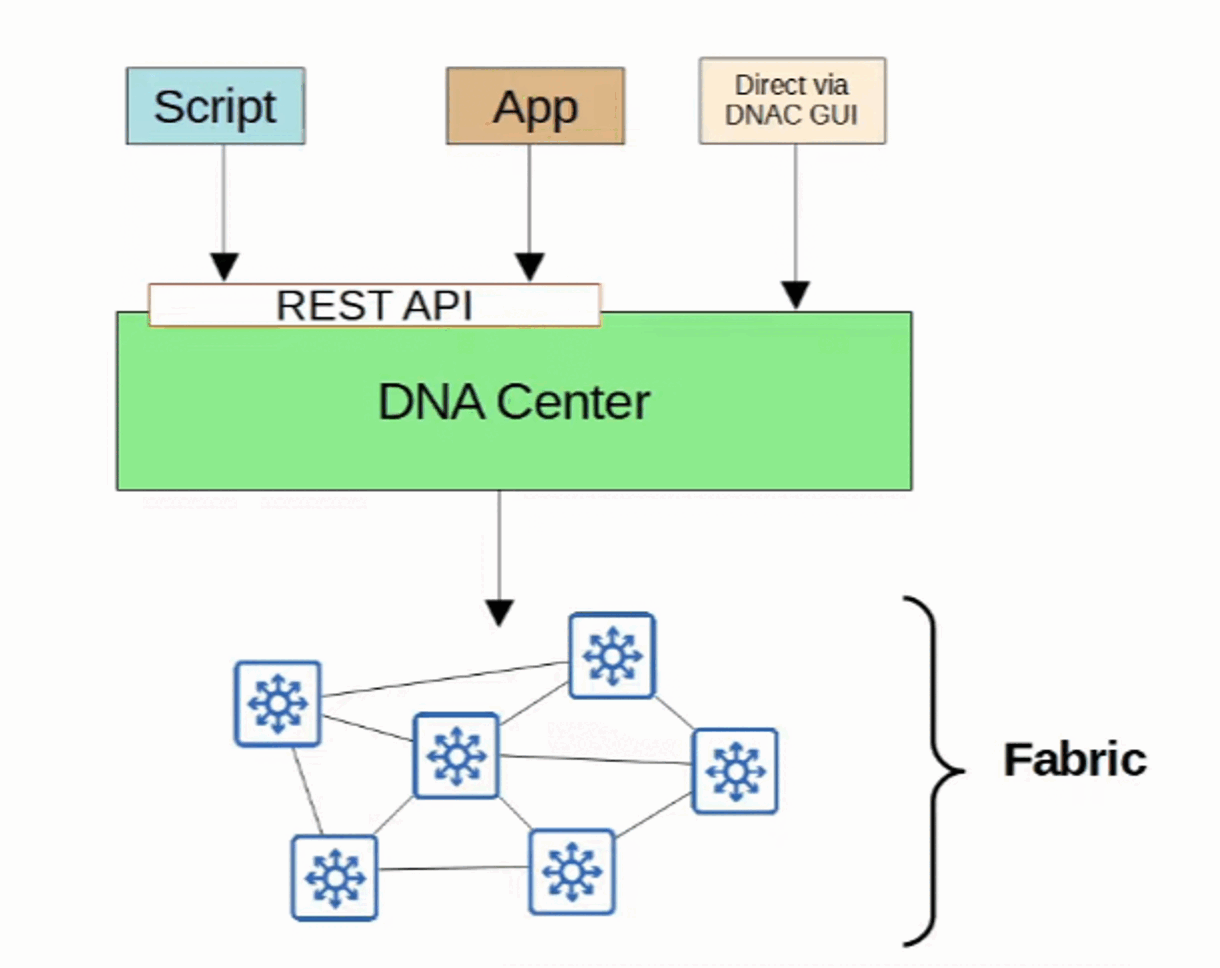
\includegraphics[keepaspectratio,alt={image}]{images/65-software-defined-networking/img-002.png}}
\end{figure}

\begin{itemize}
\tightlist
\item
  The UNDERLAY is the underlying physical network of devices and
  connections (including wired and wireless) which provide IP
  connectivity (ie: using IS-IS)

  \begin{itemize}
  \tightlist
  \item
    Multilayer Switches and their connections
  \end{itemize}
\end{itemize}

\begin{figure}
\centering
\pandocbounded{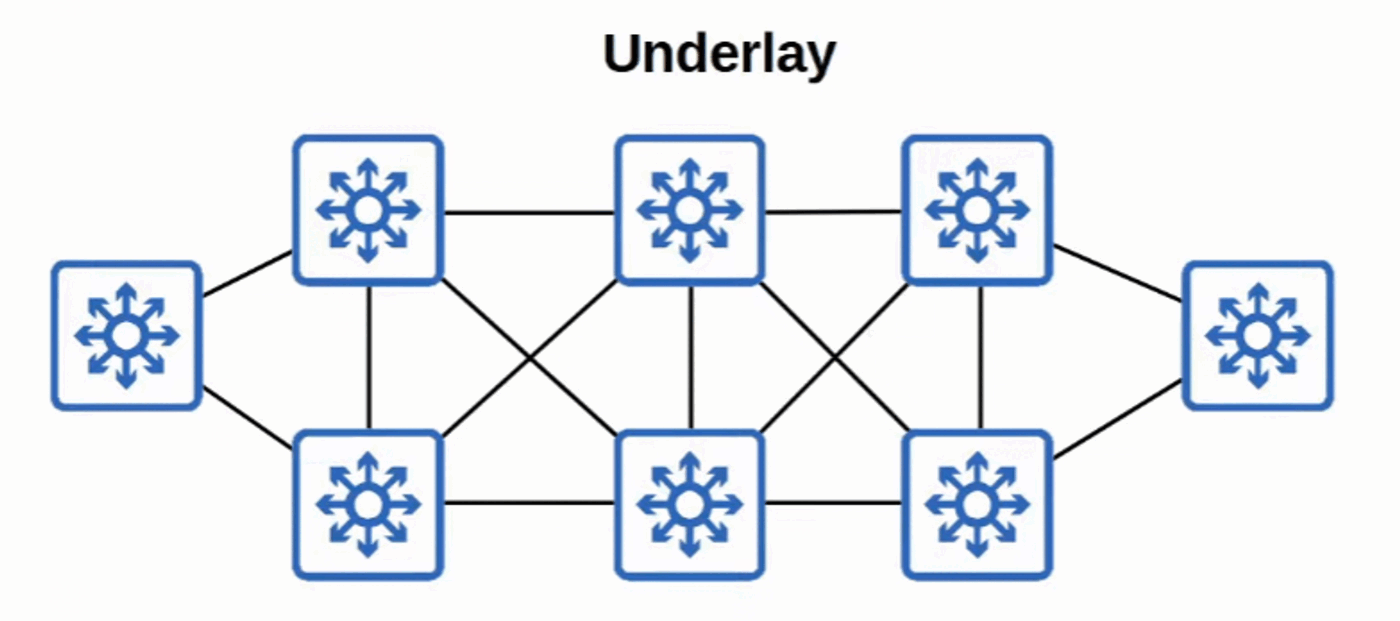
\includegraphics[keepaspectratio,alt={image}]{images/65-software-defined-networking/img-003.png}}
\end{figure}

\begin{itemize}
\tightlist
\item
  The OVERLAY is the virtual network built on top of the physical
  underlay network
\end{itemize}

\begin{figure}
\centering
\pandocbounded{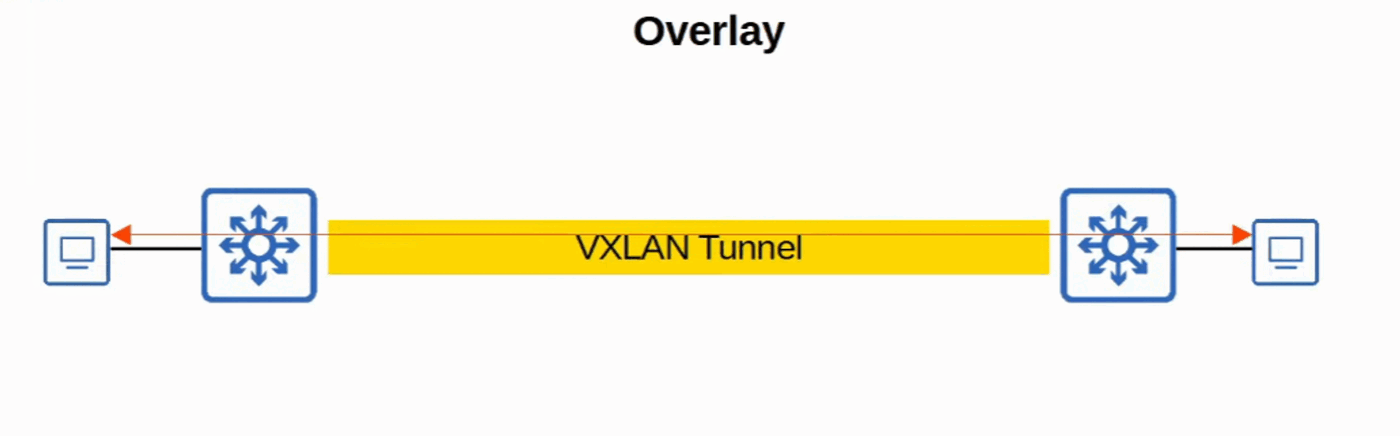
\includegraphics[keepaspectratio,alt={image}]{images/65-software-defined-networking/img-004.png}}
\end{figure}

\begin{itemize}
\tightlist
\item
  The FABRIC is the combination of the OVERLAY and UNDERLAY; the
  physical and virtual network as a whole
\end{itemize}

\begin{figure}
\centering
\pandocbounded{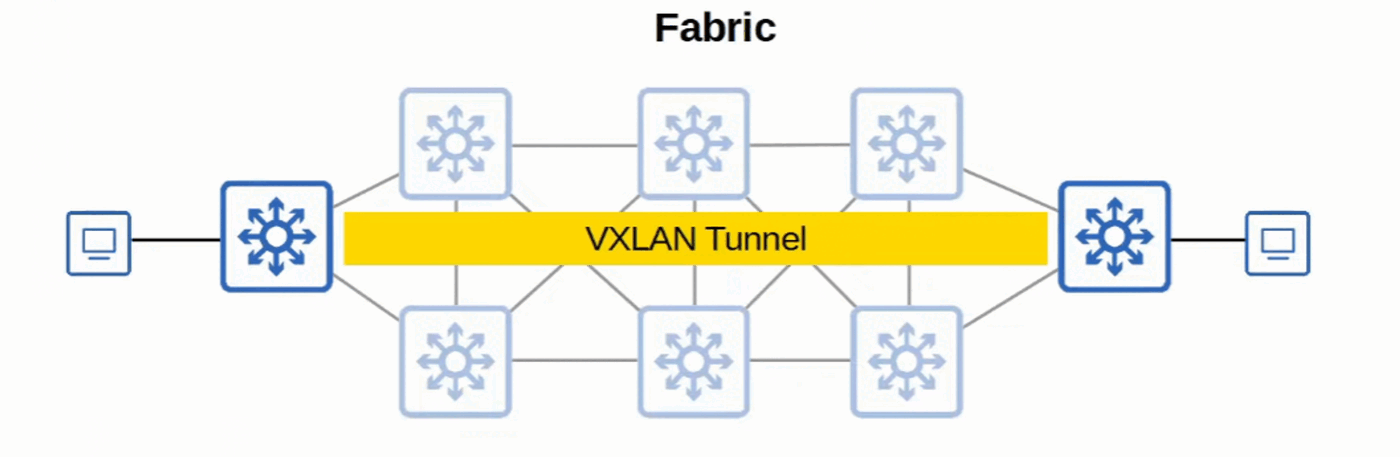
\includegraphics[keepaspectratio,alt={image}]{images/65-software-defined-networking/img-005.png}}
\end{figure}

\section{SD-Access Underlay}\label{sd-access-underlay}

\begin{itemize}
\tightlist
\item
  The UNDERLAY's purpose is to support the VXLAN tunnels of the OVERLAY
\item
  There are THREE different ROLES for switches in SD-ACCESS:

  \begin{itemize}
  \tightlist
  \item
    EDGE NODES : Connect to End HOSTS
  \item
    BORDER NODES : Connect to devices outside of the SD-ACCESS Domain ;
    ie: WAN routers
  \item
    CONTROL NODES : Uses LISP (Locator ID Separation Protocol) to
    perform various control plane functions
  \end{itemize}
\item
  You can add SD-ACCESS on top of the existing network (\emph{brownfield
  deployment}) if your network hardware and software supports it

  \begin{itemize}
  \tightlist
  \item
    Google `Cisco SD-ACCESS compatibility matrix' if you are curious
  \item
    In this case DNA CENTER won't configure the UNDERLAY
  \end{itemize}
\item
  A NEW deployment (\emph{greenfield deployment)} will be configured by
  DNA CENTER to use the optimal SD-ACCESS UNDERLAY:

  \begin{itemize}
  \tightlist
  \item
    ALL Switches are LAYER 3 and use IS-IS as their ROUTING PROTOCOL
  \item
    All Links between Switches are ROUTED PORTS. This means STP is not
    needed
  \item
    EDGE NODES (ACCESS SWITCHES) act as the the DEFAULT GATEWAY of END
    HOSTS \emph{(Routed Access Layer)}
  \end{itemize}
\end{itemize}

\begin{figure}
\centering
\pandocbounded{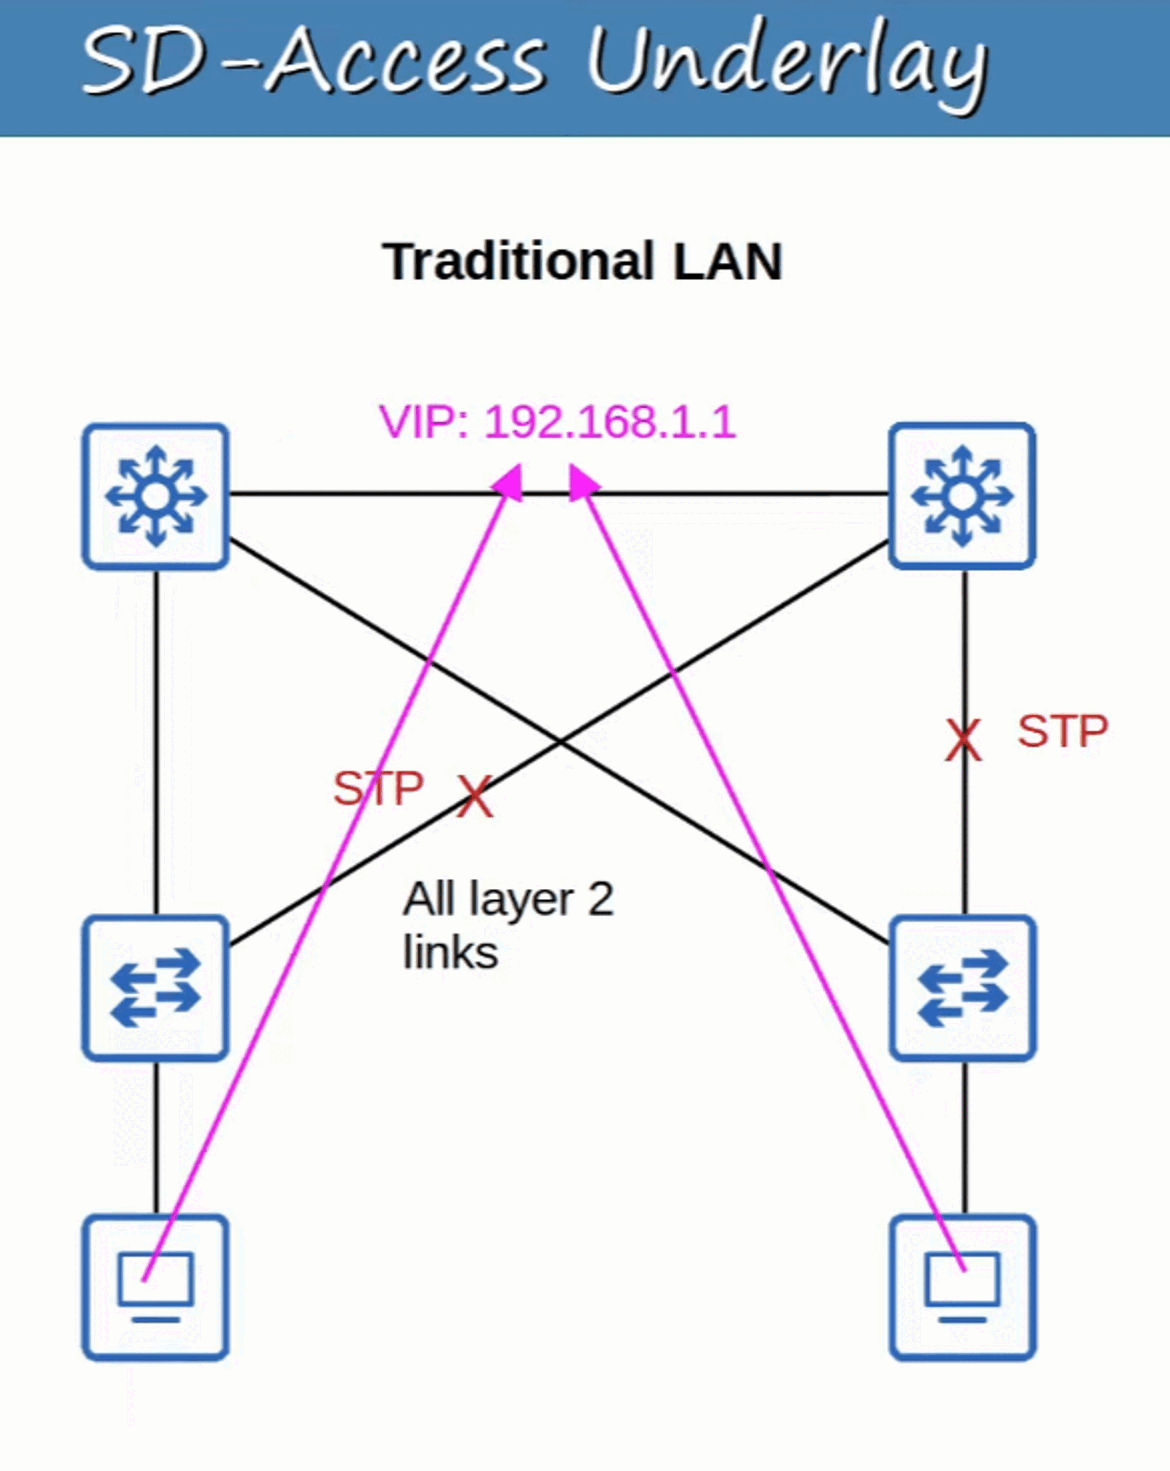
\includegraphics[keepaspectratio,alt={image}]{images/65-software-defined-networking/img-006.png}}
\end{figure}

\begin{figure}
\centering
\pandocbounded{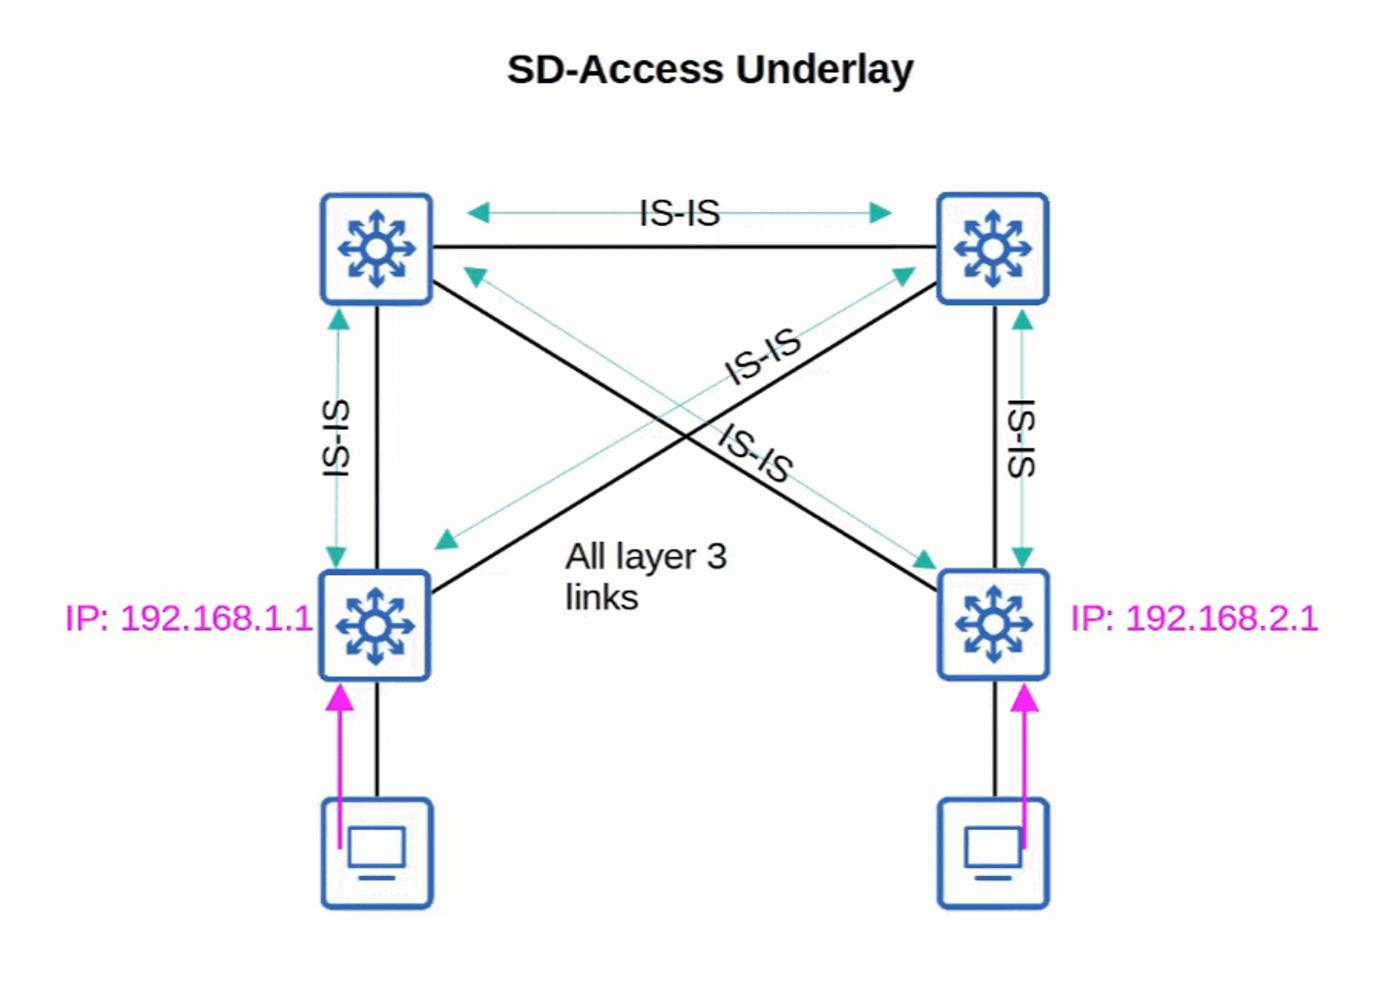
\includegraphics[keepaspectratio,alt={image}]{images/65-software-defined-networking/img-007.png}}
\end{figure}

\section{SD-Access Overlay}\label{sd-access-overlay}

\begin{itemize}
\item
  LISP (Locator ID Separation Protocol) provides the control plane of
  SD-ACCESS

  \begin{itemize}
  \tightlist
  \item
    A list of mappings of EIDs (endpoint identifiers) to RLOCs (routing
    locators) is kept
  \item
    EIDs identify END HOSTS connected to EDGE SWITCHES
  \item
    RLOCS identify the EDGE SWITCH which can be used to reach the END
    HOST
  \item
    There is a LOT more detail to cover about LISP but I think you can
    see how it differs from traditional CONTROL PLANE
  \end{itemize}
\item
  Cisco TrustSec (CTS) provides policy control (QoS, Security Policy,
  etc.)
\item
  VXLAN provides the DATA PLANE of SD-ACCESS
\end{itemize}

\begin{figure}
\centering
\pandocbounded{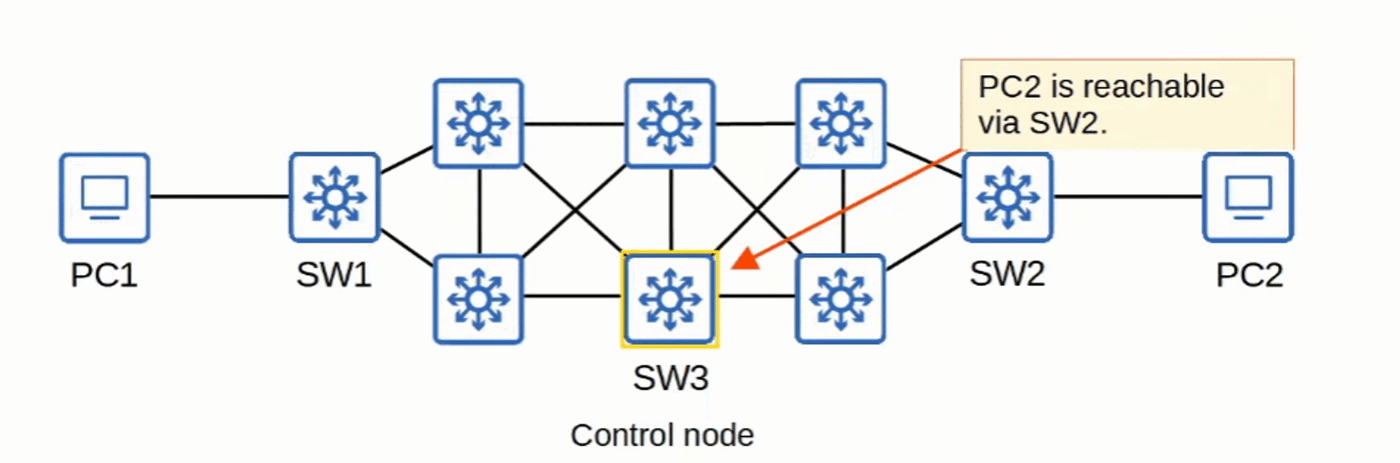
\includegraphics[keepaspectratio,alt={image}]{images/65-software-defined-networking/img-008.png}}
\end{figure}

\begin{figure}
\centering
\pandocbounded{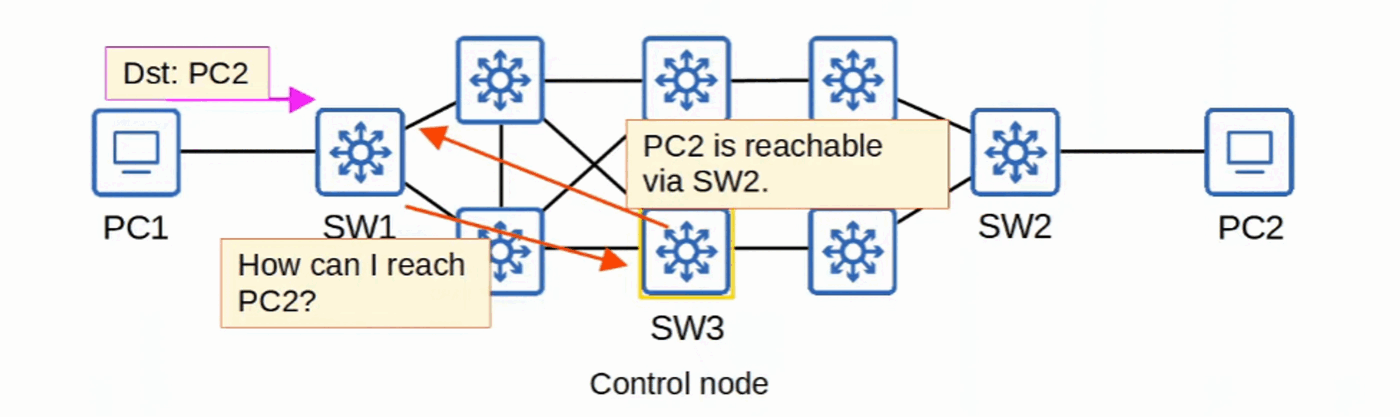
\includegraphics[keepaspectratio,alt={image}]{images/65-software-defined-networking/img-009.png}}
\end{figure}

\begin{figure}
\centering
\pandocbounded{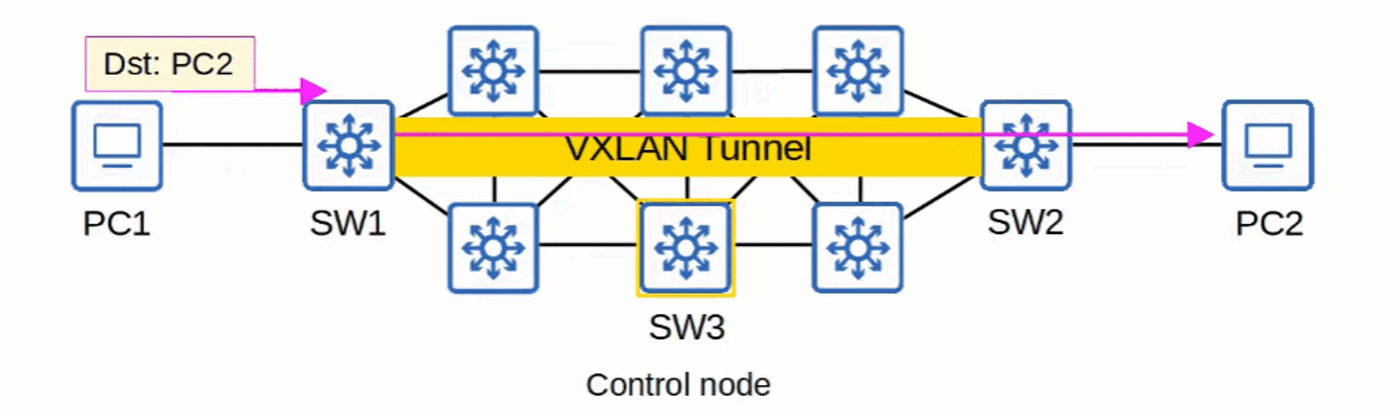
\includegraphics[keepaspectratio,alt={image}]{images/65-software-defined-networking/img-010.png}}
\end{figure}

\section{Cisco DNA Center}\label{cisco-dna-center}

\begin{itemize}
\tightlist
\item
  Cisco DNA Center has TWO MAIN ROLES:

  \begin{itemize}
  \tightlist
  \item
    The SDN Controller in SD-ACCESS
  \item
    A network manager in a traditional network (non-SD-ACCESS)
  \end{itemize}
\item
  DNA Center is an application installed on Cisco UCS server hardware
\item
  It has a REST API which can be used to interact with DNA Center
\item
  The SBI supports protocols such as NETCONF and RESTCONF (as well as
  traditional protocols like Telnet, SSH, and SNMP)
\item
  DNA Center enables \emph{Intent-Based Networking} (IBN)

  \begin{itemize}
  \tightlist
  \item
    The goal is to allow the engineer to communicate their intent for
    network behavior to DNA Center, and then DNA Center will take care
    of the details of the actual configurations and policies on devices
  \end{itemize}
\item
  Traditional security policies using ACLs can become VERY cumbersome

  \begin{itemize}
  \tightlist
  \item
    ACLs can have thousands of entries
  \item
    The intent of entries is forgotten with time and as engineers leave
    and new engineers take over
  \end{itemize}
\item
  DNA Center allows the engineer to specify the intent of the policy

  \begin{itemize}
  \tightlist
  \item
    Examples :

    \begin{itemize}
    \tightlist
    \item
      THIS group of users can't communicate with THAT group
    \item
      THIS group can access THIS server but not THAT server
    \end{itemize}
  \item
    DNA CENTER will take care of the exact details of implementing this
    policy
  \end{itemize}
\end{itemize}

\begin{figure}
\centering
\pandocbounded{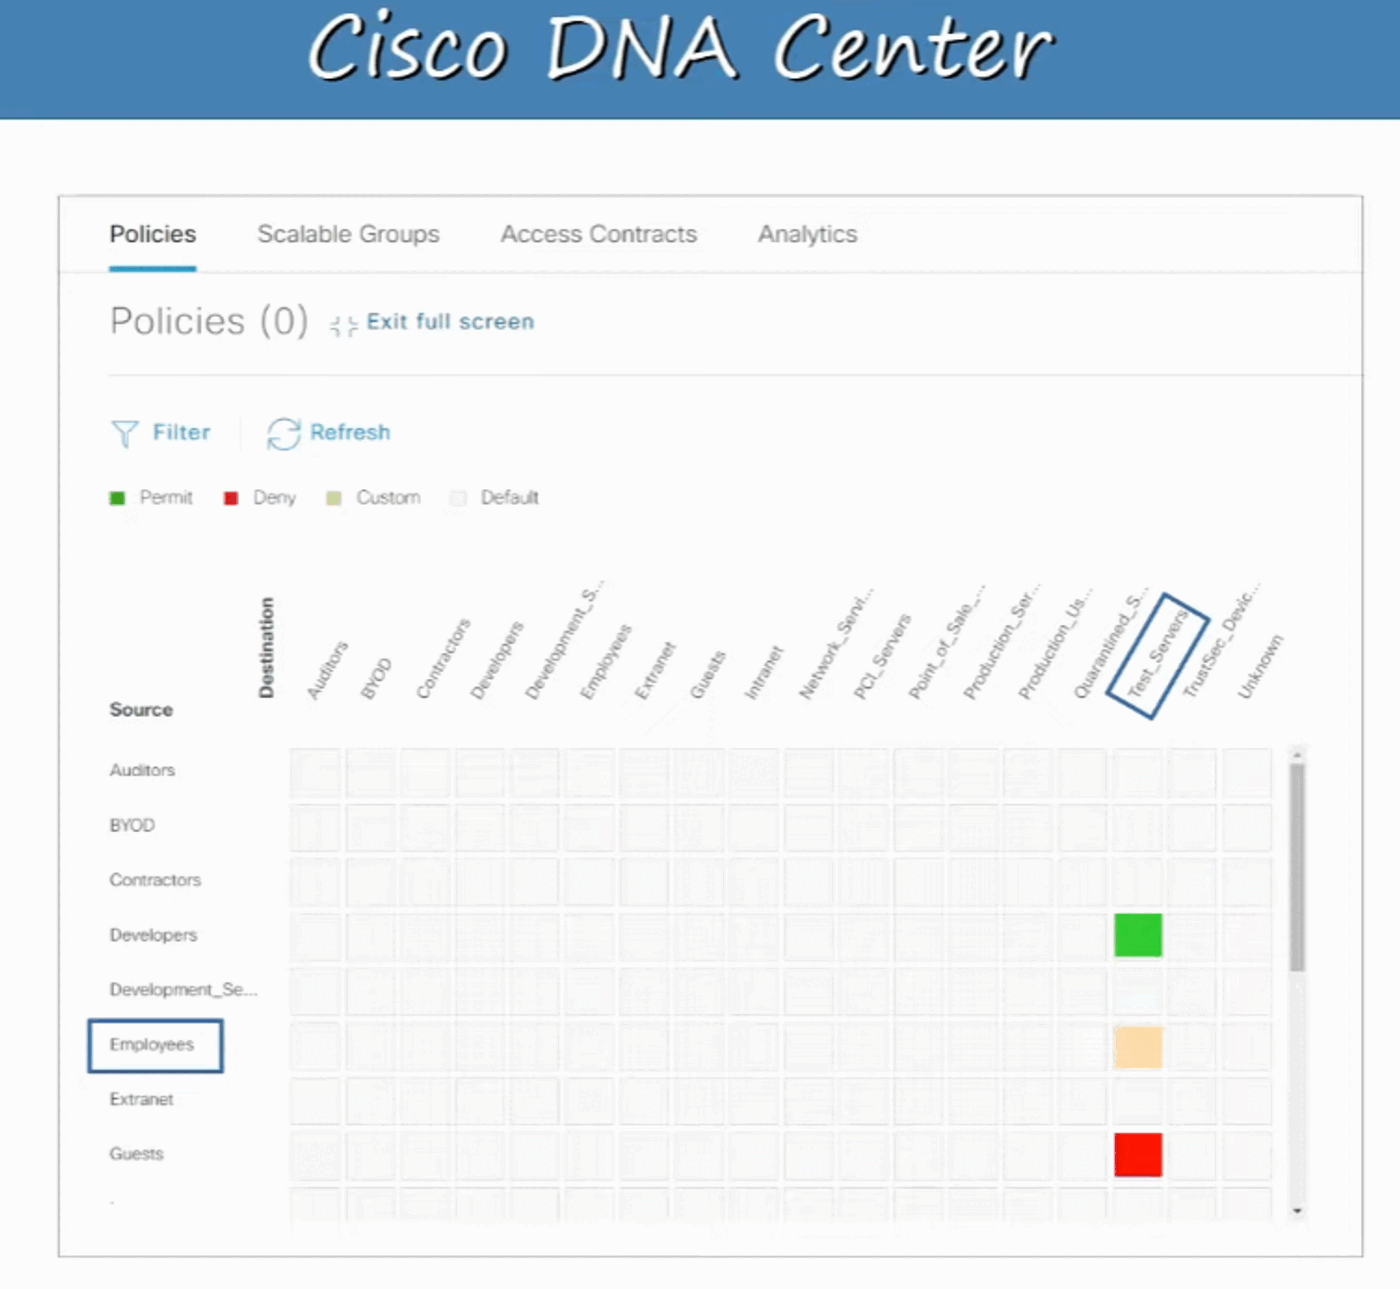
\includegraphics[keepaspectratio,alt={image}]{images/65-software-defined-networking/img-011.png}}
\end{figure}

\begin{quote}
For more details, you can check out
\href{http://sandboxdnac.cisco.com}{sandboxdnac.cisco.com} (User:
devnetuser, Password: Cisco123!)
\end{quote}

\section{DNA Center Network Management Vs.
Traditional}\label{dna-center-network-management-vs.-traditional}

Traditional Management :

\begin{itemize}
\tightlist
\item
  DEVICES are configured one-by-one via SSH or Console connection
\item
  DEVICES are manually configured via Console connection before being
  deployed
\item
  Configurations and polices are managed per-device
\item
  New network deployments can take a long time due to the manual labor
  required
\item
  Errors and failures are more likely due to increased manual effort
\end{itemize}

DNA CENTER-based Network Management :

\begin{itemize}
\tightlist
\item
  DEVICES are centrally managed and monitored from the DNA CENTER GUI or
  other applications using it's REST API
\item
  The Administrator communicates their intended network behavior to DNA
  CENTER, which changes those intentions into configurations on the
  managed network devices
\item
  Configurations and policies are centrally managed
\item
  Software versions are also centrally managed. DNA CENTER can monitor
  cloud servers for new versions and then update the managed devices
\item
  New network deployments are much quicker. New devices can
  automatically receive their configurations from DNA CENTER without
  manual configuration
\end{itemize}

\begin{figure}
\centering
\pandocbounded{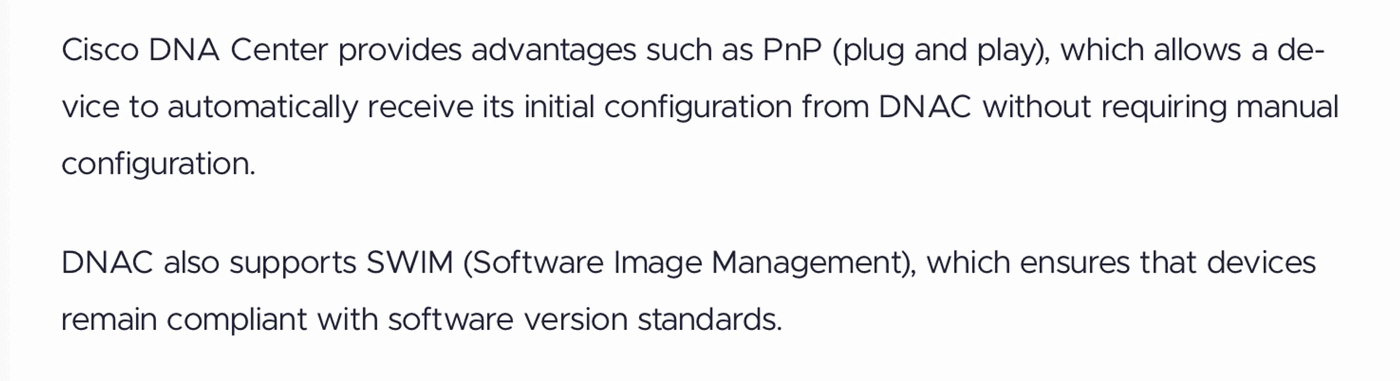
\includegraphics[keepaspectratio,alt={image}]{images/65-software-defined-networking/img-012.png}}
\end{figure}
